\chapter{Fine-grain Parallelization of SKPDP}
\label{chap:finegrain}

%We explore two parallelization strategies, Coarse-grain and Fine-grain. In the Coarse-grain parallelization strategy, a processor is responsible for computing an entire row in the table.  Whereas in the Fine-grain parallelization strategy, all processors contribute to the computation of a row.

%\subsection{Coarse-grain Parallelization}
%ABCD

%\subsection{Fine-grain Parallelization}
In fine-grain parallelism, the computation of a single row is equally distributed amongst $P$ processors or threads (except the last processor which might have less number of elements to compute).  Every row in the sparse table has a different size.  If the size of the row is less than $P*w_{i}*\alpha$, then the row is computed by a single processor (or thread).  Here,  $\alpha$ is a constant greater than $2$.  Once the size of the row exceeds the threshold of $P*w_{i}*\alpha$, the row is equally split into $P$ sections with contiguous elements such that the $i_{th}$ processor is responsible for computing the $i_{th}$ section of the row.  The size of each section is $C/P$, where the last processor might have less number of elements to compute.  All processors independently compute their respective sections in parallel.  When all processors have finished computing, the sections are then stitched together using a mechanism similar to the \emph{Merge-kill} mechanism explained in section \ref{sec:merge-kill}.  
%This stitching is performed by a single processor.  
Additionally, the elements are sorted by the decreasing order of their weights.  This means the element with the maximum weight is computed first and the element with the minimum weight is computed at the end.  This allows for $P$ processors to start computing rows in parallel from a certain point in the table and continue parallel execution henceforth.  


\begin{figure}[htbp]
\centerline{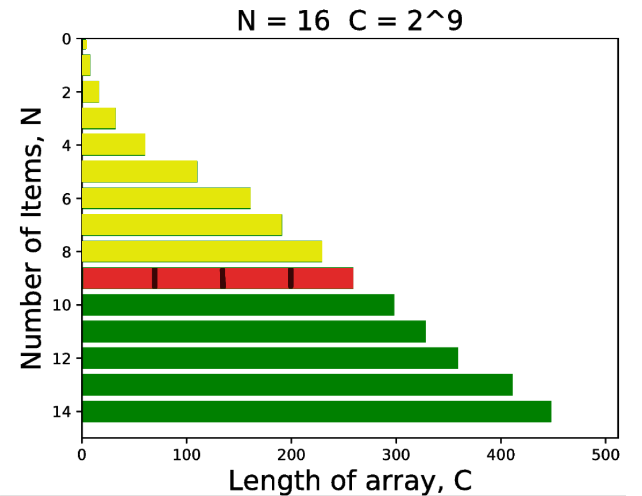
\includegraphics[width=0.8\columnwidth]{images/finegrain.png}}
\caption{Fine-Grain Parallelization. }
\label{fig:finegrain}
\end{figure}

As shown in Figure \ref{fig:finegrain},  the fine-grain parallel computation begins at the red row where the size of the row is greater than $P*w_{i}*\alpha$.  The  row is split into $P$ sections, each section has a starting index and a ending index.  A processor (or a thread) computes its section while reading the elements from previous row and produces a current/output buffer.  All the threads execute in parallel and produce an output buffer.  These output buffers then have to be merged in order to produce the output row.  Note that some of the values produced by the output buffer of the processor $P_i$ may be dominated by the elements in the output buffer of the processor $P_{i+1}$. The suffix of the output buffer of the processor $P_i$ will have an overlap with the prefix of the output buffer of the processor $P_{i+1}$.  The output buffers therefore need to be stitched together and more work is needed.  For the stitching, all the threads (in parallel) eliminate dominating values from their suffix and produce a merged output row.  The threads move on to the next row after stitching.

\section{Overhead Analysis} 
The extra work involved in the stitching can slow down the computation.  The maximum overlap between any two threads can be of the size of $2w_i$. Note that the size of the row must be greater than $2P*w_{i}*\alpha,\text{where } \alpha>2$.  This ensures that there cannot be any overlap between the processors $P_{i-1}$ and $P_{i+1}$ while stitching.  In the worst case, $2w_i$ elements will need to be merged for every section for every row.  This means that a total of $2P* \sum_i w_i$ extra computation must be performed for stitching the output row.  The upper bound on $2P* \sum_i w_i$ is $C$, the capacity.  Every row will do $C$ extra work, at worst.  This means a total of $N'*C, \text{where } N'=\text{number of rows calculated using this technique and } N' < N$, extra work is needed which can be double the work compared to sequential version.



\section{Implementation Details} 
In our implementation, we do not try to parallelize the sparse rows that are too small according to the following criterion,

\begin{equation}
\label{eq: fine-grained-criteria}
l_{i-1} > \alpha P w_i
\end{equation}
where $l_{i-1}$ is length of the last calculated sparse row $S_{i-1}$. \\
Once a sparse row $S_i$ is found that fulfills the criterion (\ref{eq: fine-grained-criteria}) we apply our fine-grained parallelization technique on all subsequent sparse rows. To ensure that the subsequent rows fulfill the criterion (\ref{eq: fine-grained-criteria}) too we sort the items by descending values of weight so that the right hand side of (\ref{eq: fine-grained-criteria}) is non-increasing. But, the problem is that length of the sparse rows are not non-decreasing, which can cause the the criterion (\ref{eq: fine-grained-criteria}) to fail for subsequent sparse rows. So, our current implementation is not flawless.


\section{Results}
Due to high overhead of achieving the fine-grained parallelization, this technique performs a constant factor worse than the sequential version. But due to the flaw in our implementation the results are not completely reliable. 




